\section{Background}
    \subsection{Stato dell'arte}

    \begin{frame}{\insertsectionhead}{\insertsubsectionhead}

      % \subsubsection{Programmazione aggregata}
      \begin{block}{Programmazione aggregata} % \insertsubsubsectionhead
        La programmazione aggregata costituisce un'alternativa all'approccio ``classico'' volta a semplificare la progettazione, creazione e manutenzione di sistemi distribuiti complessi.
      \end{block}

      \pause

      % \subsubsection{Linguaggi}
      \begin{block}{Linguaggi} % \insertsubsubsectionhead
        I principali linguaggi di programmazione aggregata sono:

        \begin{itemize}[<+(1)->]
          \item ScaFi
          \item Protelis
        \end{itemize}
      \end{block}

    \end{frame}

    \begin{frame}{\insertsectionhead}{\insertsubsectionhead}

      % TODO: inserisci il logo

      \begin{block}{Protelis}
        \begin{itemize}[<+->]
          % TODO: non è chiaro da dove salti fuori field calculus qua
          \item Field calculus è un impianto teorico sul quale devono essere costruiti linguaggi ``pratici''.
          % TODO: abbrevia
          \item \strong{Protelis} è un linguaggio di programmazione basato sul paradigma aggregato fortemente influenzato da \emph{Proto}.
          % TODO: abbrevia
          \item Il linguaggio incorpora le principali funzionalità di computazione spaziale di field calculus in una sintassi più simile ai linguaggi strutturati tradizionali come C o Java.
        \end{itemize}
      \end{block}
    \end{frame}

    \subsection{Problematiche}

    \begin{frame}{\insertsectionhead}{\insertsubsectionhead}

      \begin{block}{\insertsubsectionhead}
        \begin{itemize}[<+->]
          \item
            Il linguaggio è \emph{Java-hosted}
            \begin{itemize}
              \item richiede un ambiente JVM in cui eseguire l'interprete
            \end{itemize}
          \item
            Il linguaggio richiede una rete di dispositivi su cui eseguire
            \begin{itemize}[<+->]
              \item rete fisica
              \item NASA WorldWind  % TODO: figura
              \item ProtelisVM      % TODO: figura
              \item Alchemist       % TODO: figura
            \end{itemize}
        \end{itemize}
      \end{block}
    \end{frame}

    \subsection{Requisiti e casi d'uso}

    \begin{frame}{\insertsectionhead}{\insertsubsectionhead}

      \begin{block}{Requisiti}
        \begin{itemize}
          \item
            L'obiettivo è progettare un sistema che permetta all'utente di iniziare a utilizzare Protelis richiedendo meno configurazioni possibile.
            \begin{itemize}
              \item nessun build-script
              \item nessuna rete o simulatore
            \end{itemize}
          \item
            l'utente si assume essere inesperto della piattaforma
            \begin{itemize}
              \item l'interfaccia deve essere semplice e immediata
            \end{itemize}
        \end{itemize}
      \end{block}

      % TODO: figure aside
    \end{frame}

    \begin{frame}{\insertsectionhead}
      \framesubtitle{\insertsubsectionhead}

      \begin{block}{Fattibilità}
        \begin{itemize}
          \item
            non è possibile eseguire un interprete Protelis all'interno della sandbox un browser
            \begin{itemize}
              \item le Java applet sono deprecate da tempo
            \end{itemize}
          \item
            è necessario suddividere l'architettura in due componenti
            \begin{itemize}
              \item un server che espone API per l'esecuzione del codice
              \item un'interfaccia Single-Page accessibile tramite browser
            \end{itemize}
        \end{itemize}
      \end{block}

      \begin{figure}
        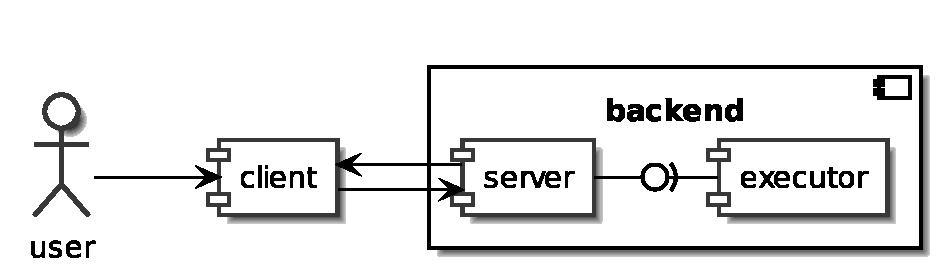
\includegraphics[width=.8\textwidth]{../res/uml/architecture-design.eps}
      \end{figure}

      % TODO: figure aside
    \end{frame}

